% !TEX root = main.tex

\section{Related Works}

A popular design choice for image captioning systems involves using a
convolutional neural network (CNN) as the image encoder and a recurrent neural
network (RNN) with a closed vocabulary as a decoder~\cite{Karpathy2015DeepVA,
   Donahue2015LongTR, Vinyals2015ShowAT}. Attention over image patches using a
multilayer perception was introduced in ``Show, Attend and Tell"
\cite{Xu2015ShowAA}. Further extensions include having the option to not attend
to any image region~\cite{Lu2017KnowingWT} using a bottom-up approach to
propose a region to attend to~\cite{Anderson2017BottomUpAT}, and attending
specifically to object regions~\cite{Wang2019Hierarchical} and visual concepts
\cite{You2016ImageCW,Li2019Boosted,Wang2019Hierarchical} identified in the
image.
% When attending to more than one modality, there
% are various strategies on how to combine embeddings such as addition,
% concatenation, and multivariate residual modules (MRMs)
% \cite{Kim2016MultimodalRL}. All of these systems can only generate generic
% captions without considering context external to the image.


% In our model we use the vector concatenation
% strategy and leave investigation of the more complex strategies, such as MMRs,
% to future work as they typically only yield minor performance
% improvements~\cite{Wang2019Hierarchical}.

% using reinforcement learning
% to directly optimise for the CIDEr metric~\cite{Rennie2017SelfCriticalST,
% Gao2019DeliberateAN}

News image captioning includes the article text as input and focuses on the
types of images used in news articles. A key challenge here is to generate
correct entity names, especially rare ones. Existing approaches include
extractive methods that use n-gram models to combine existing phrases
\cite{Feng2013AutomaticCG} or simply retrieving the most representative
sentence~\cite{Tariq2017ACE} in the article. Ramisa
\etal~\cite{Ramisa2016BreakingNewsAA} built an end-to-end LSTM decoder that
takes both the article and image as inputs, but the model was still unable to
produce names that were not seen during training.

To overcome the limitation of a fixed-size vocabulary, template-based methods
have been proposed. An LSTM first generates a template
sentence with placeholders for named entities, e.g. ``PERSON speaks at BUILDING
in DATE.''~\cite{Biten2019GoodNews}. Afterwards the best candidate for each
placeholder is chosen via a knowledge graph of entity
combinations~\cite{Lu2018EntityAI}, or via sentence
similarity~\cite{Biten2019GoodNews}. One key difference between our proposed
model and previous approaches~\cite{Biten2019GoodNews,Lu2018EntityAI}
is that our model can generate a caption with named entities directly without
using an intermediate template.

\begin{figure*}[t]
   \begin{center}
      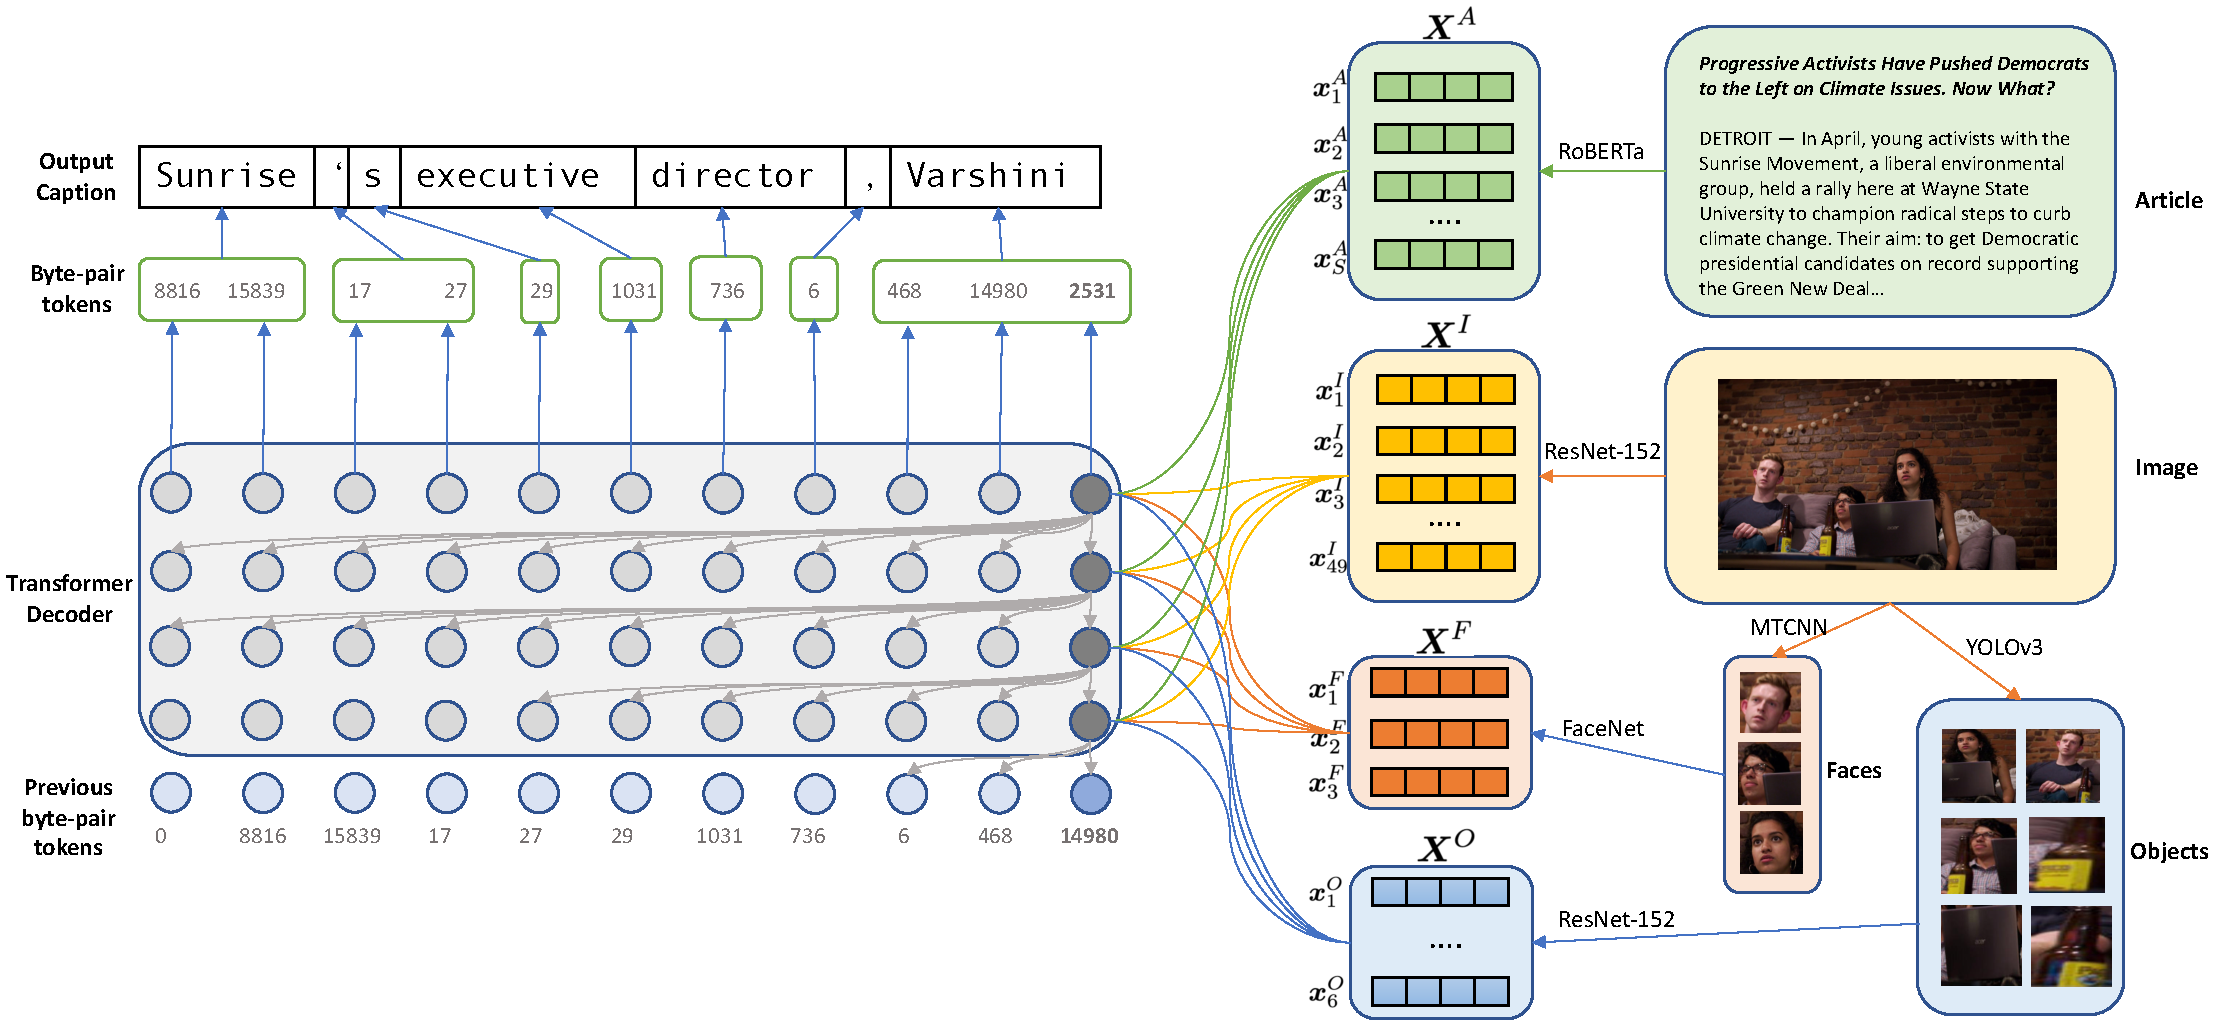
\includegraphics[width=\linewidth]{figures/figure_2.pdf}
   \end{center}

   \capmoveup
   \caption{Overview of the Transform and Tell model. Left: Decoder with four
      transformer blocks; Right: Encoder for article, image, faces, and
      objects. The decoder takes as input embeddings of byte-pair tokens (blue
      circles at the bottom). For example, the input in the final time step,
      14980, represents ``arsh'' in ``Varshini'') from the previous time step.
      The grey arrows show the convolutions in the final time step in each
      block. Colored arrows show attention to the four domains on the right:
      article text (green lines), image patches (yellow lines), faces (orange
      lines), and objects (blue lines). The final decoder outputs are byte-pair
      tokens, which are then combined to form whole words and punctuations.}
   \postfigmoveup
   \label{fig:model}
\end{figure*}

One tool that has seen recent successes in many natural language processing
tasks are transformer networks. Transformers have been shown to consistently
outperform RNNs in language modeling~\cite{Radford2019LanguageMA},
story generation~\cite{Fan2018HierarchicalNS},
summarization~\cite{Subramanian2019OnEA}, and machine
translation~\cite{Bojar2018Findings}. In particular, transformer-based models
such as BERT~\cite{Devlin2019BERT}, XLM~\cite{Lample2019CrosslingualLM},
XLNet~\cite{Yang2019XLNetGA}, RoBERTa~\cite{Liu2019RoBERTaAR}, and
ALBERT~\cite{Lan2019ALBERT} are able to produce high level text representations
suitable for transfer learning. Furthermore, using byte-pair encoding
(BPE)~\cite{Sennrich2015NeuralMT} to represent uncommon words as a sequence of
subword units enables transformers to function in an open vocabulary setting.
To date the only image captioning work that uses BPE
is~\cite{Zhao2019InformativeIC}, but they did not use it for rare named
entities as these were removed during pre-processing. In contrast we explicitly
examine BPE for generating rare names and compare it to template-based methods.

Transformers have been shown to yield competitive results in generating generic
MS COCO captions~\cite{Zhu2018CaptioningTW, Li2019Boosted}. Zhao
\etal~\cite{Zhao2019InformativeIC} have gone further and trained transformers
to produce some named entities in the Conceptual Captions
dataset~\cite{Sharma2018ConceptualCA}. However, the authors used web-entity labels, extracted using
Google Cloud Vision API, as inputs to the model. In our work, we do not
explicitly give the model a list of entities to appear in the caption. Instead
our model automatically identifies relevant entities from the provided news
article.

%We fill this gap and in particular examine how much
%better BPE can generate rare names compared to template-based methods.
